\documentclass[conference]{IEEEtran}
\IEEEoverridecommandlockouts
% The preceding line is only needed to identify funding in the first footnote. If that is unneeded, please comment it out.
\usepackage{cite}
\usepackage{amsmath,amssymb,amsfonts}
\usepackage{algorithmic}
\usepackage{graphicx}
\usepackage{textcomp}
\usepackage{xcolor}
\usepackage{listings}
\usepackage{hyperref}
\hypersetup{
    colorlinks=true,
    linkcolor=blue,
    filecolor=magenta,      
    urlcolor=cyan,
}
\def\BibTeX{{\rm B\kern-.05em{\sc i\kern-.025em b}\kern-.08em
    T\kern-.1667em\lower.7ex\hbox{E}\kern-.125emX}}
\begin{document}

\title{RBE595 Proposal\\
{\footnotesize \textsuperscript{}Discovering Novel Swarm Behaviors through Color and Robot Capabilities
% So this line above is important for formatting, otherwise the last page ends up getting messed up with references separated across both columns with images in nonsensical locations
}
\thanks{Identify applicable funding agency here. If none, delete this.}
}

\author{\IEEEauthorblockN{Claypool}
\IEEEauthorblockA{\textit{Computer Science} \\
\textit{Worcester Polytechnic Institute}\\
Worcester, USA \\
smclaypool@wpi.edu}
\and
\IEEEauthorblockN{Enyedy}
\IEEEauthorblockA{\textit{Robotics Engineering} \\
\textit{Worcester Polytechnic Institute}\\
Worcester, USA \\
ajenyedy@wpi.edu}
\and
\IEEEauthorblockN{Hosea}
\IEEEauthorblockA{\textit{Robotics Engineering} \\
\textit{Worcester Polytechnic Institute}\\
Worcester, USA \\
rdhosea@wpi.edu}
}

\maketitle

\begin{abstract}
Emergent behavior research in swarms has primarily been based on binary proximity sensors. This research has provided a list of emergent behaviors that can be expected from simple, evolving swarm systems. 
We base our research on the work outlined in Brown et al. \cite{c1}, which describes the process of discovering which emergent behaviors can occur given a limited capability model of a robot.
We plan to expand on their research by adding a color to each robot representing a heterogeneous `type', and changing the binary sensor to an N-bit sensor detecting the color of the visible robots where N is the total number of colors.
Our goal is to determine if, given this simple capability model, these robots can exhibit self-segregation based on their color. 

\end{abstract}

\section{Introduction}
Swarm systems have a variety of applications which are starting to beginning to become possible with modern technology. Tasks such as construction, exploring, search and rescue. 
Often, these tasks are implemented by trying to create a set of rules to control a swarm, or predicting the behavior of a swarm given a set of rules. 
Brown et. al. take a different approach, instead asking "given a set of \emph{capabilities}, what are the possible emergent behaviors that can occur?". 
This is an important question as it provides a lower-bound for defining the required complexity for a robot in a swarm to observe a desired emergent behavior. 

In nature, the emergent behavior of ``self-segregation'' is often important for creating complex behaviors from heterogeneous structures. 
For example, cockroaches exhibit preferential aggregation based on their smell \cite{c2}.
Ants also exhibit a form of self-segregation when organizing their young - ant brood that require more attention or food are placed on the perimeter to allow for easy-access whereas ants that do not require attention are placed in the center. \cite{c3}.
Segregation is also present at the molecular level accounting for phenomena such as organ formation. 

Previous research has been done to model the segregation of robots based on role. 
One approach to this is to apply a ``differential adhesivity'' model where heterogeneous types of robots exhibit a different levels of adhesion and cohesion based on their type \cite{c4}.
This model takes inspiration from the mechanisms that allow cell types to self-segregate in biological systems. 
Other models have been created that determine if self-segregation is possible through limited capability models and simple `if-then-else' statements with a similar goal of defining a complexity lower-bound for self-segregation \cite{c5}.

We propose a solution to this problem using a capability model similar to Brown et. al. where each robot has a differential drive motor controlled by a shallow neural network. 
We augment that capability model of Brown et. al. by adding a `color' parameter to each robot, and changing the binary line-of-site sensor to an N-bit sensor reporting the color of the observed robot. 
Our goal is to determine whether a swarm of robots can develop self-segregation behavior based on this limited capability model.


\section{Proposed Work}
We propose a system using simple differential drive robots as described in Brown et al. \cite{c1} and shown in Fig. \ref{bot_fig}, but with the added capabilities of sensing colors and defining their colors.
This color field for each robot will be implemented as a 1-hot encoded vector.
Initially, this color field will simply be a 2 bit vector as we will initially test just two groups of robots. 
The sensor will be adjusted to report an N-bit vector corresponding to the color of the robot seen. 
In the case that not robot is in the line of sight of the sensor, it will report a vector of all zeroes. 
To simplify the neural network, we will have collapse the input into 2 bits regardless of the number of classes in the simulation. 
The first bit will be a 1 if a robot of the same type is detected by the sensor, and the second bit will be a 1 if a robot of the second type is detected by the sensor. 
This new configuration can be seen in Figure~\ref{fig:nnet}


\begin{figure}
    \centering
    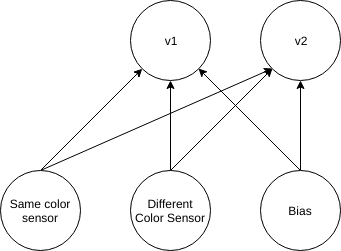
\includegraphics[width=\linewidth]{nnet.png}
    \caption{Neural Network Controller}
    \label{fig:nnet}
\end{figure}

\begin{figure}
    \centering
    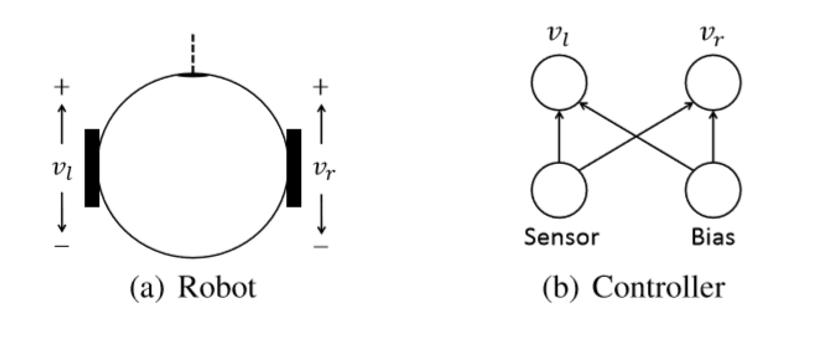
\includegraphics[width=\linewidth]{diff_drive_robot.PNG}
    \caption{Robot model from \cite{c1}}
    \label{bot_fig}
\end{figure}



\section{Proposed Experiments and Expected Outcomes}

\begin{figure}
    \centering
    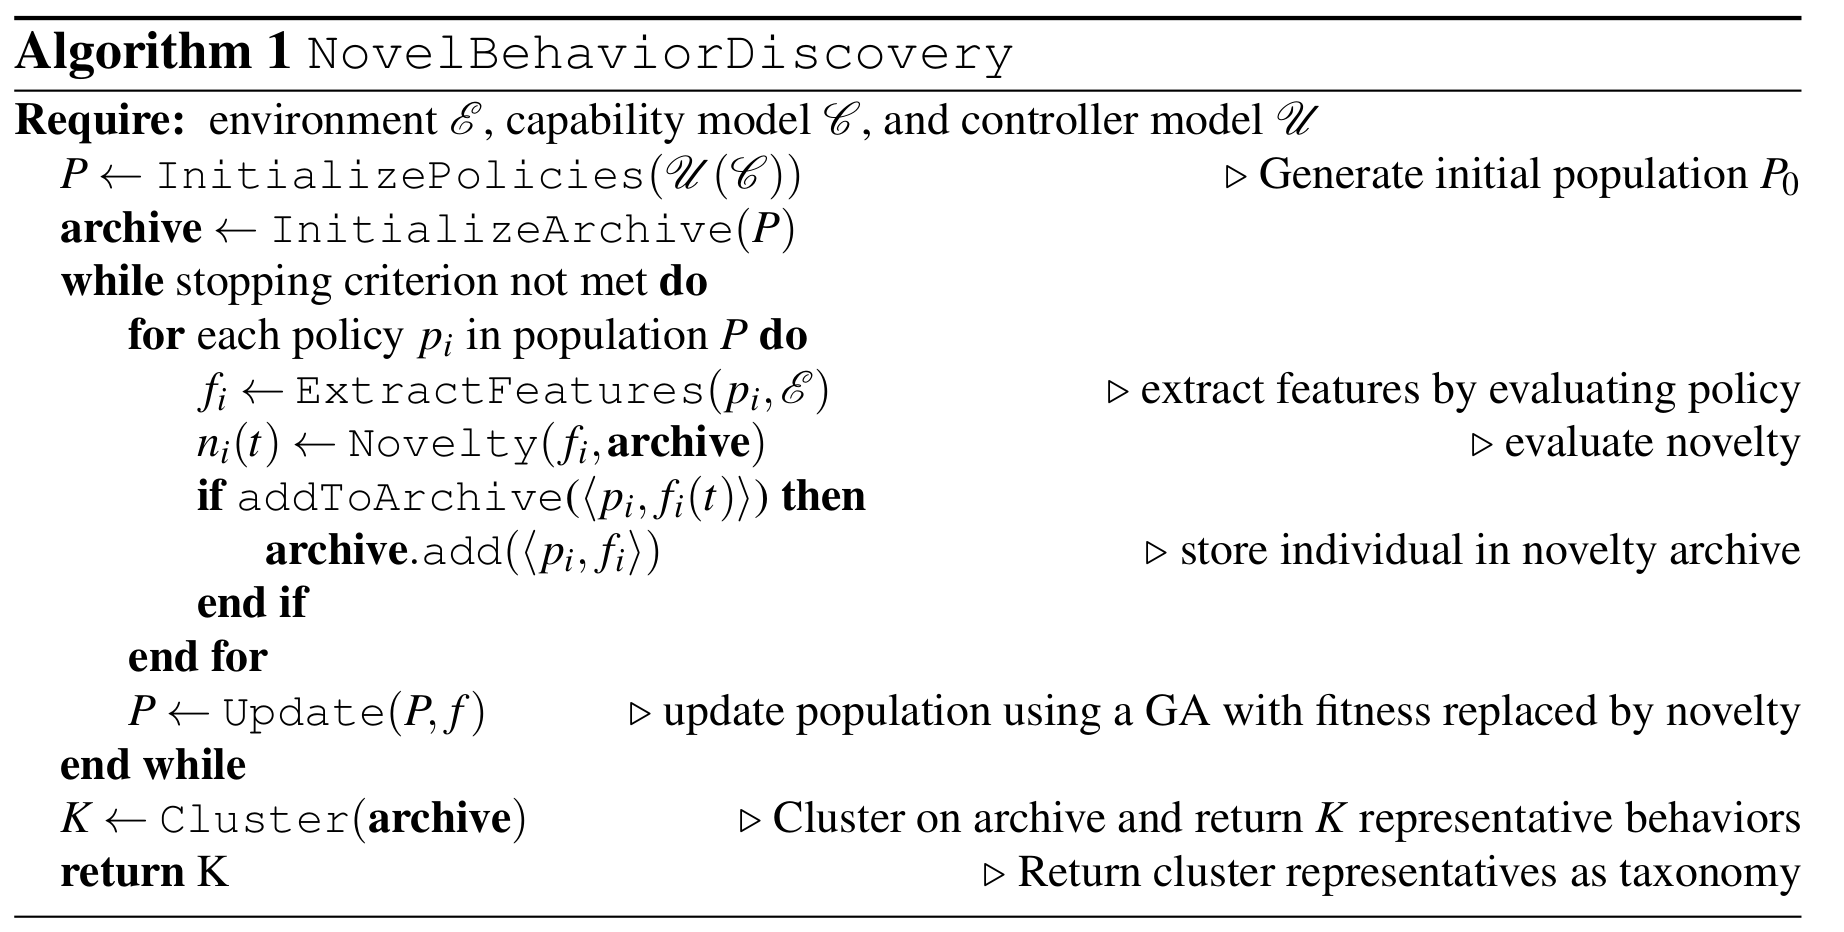
\includegraphics[width=\linewidth]{alg.png}
    \caption{Novelty search as seen in \cite{c1}}
    \label{fig:alg}
\end{figure}


We will follow a similar construction to Brown et. al. to test our hypothesis. 
We will perform an evolutionary search over the possible neural network states and prioritize novel behaviors, as described in Figure~\ref{fig:alg}. 

Rather than clustering the observed statistics through unsupervised methods such as K-medoids, we will rank our observed behaviors using a measure of segregation, such as the intersection of convex hulls based on Santos et. al.~\cite{c6}.
The intersection of convex hulls summarizes the convex shape of each cluster of robots as a convex hull, and measures the overlap between the different classes.
This means that, if the classes are each perfectly separated, there will be no overlap between the nulls of each class, so the overlap will be zero. 

Once we can rank the models by their separation, we will visually inspect the top results to categorize their behavior and separation mechanisms. 

\section{Weekly Schedule}
To complete our objectives, we will have weekly meetings on both Tuesdays and Wednesdays at 6pm. At these meetings we will convene to review our progress over the past week and plan our work for the upcoming week. 
We set up a Gantt chart to plan our weekly progress, shown in Figure~\ref{fig:gantt_chart}
\begin{figure}
    \centering
    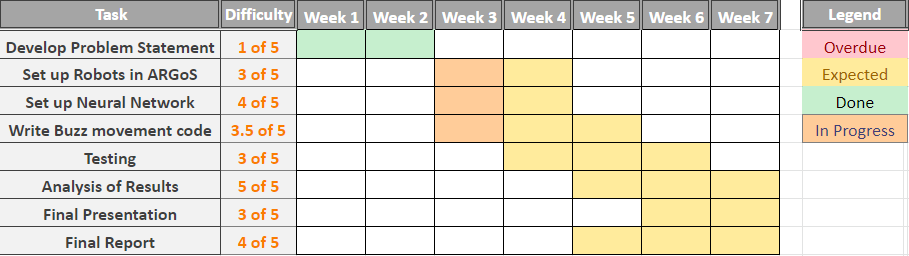
\includegraphics[width=\linewidth]{gantt_chart.PNG}
    \caption{Gantt Chart}
    \label{fig:gantt_chart}
\end{figure}


\section{Implementation}
\label{sec:imp}

\subsection{Individual Argos Simulations}

We use Argos to virtually test different neural network weight configurations, as described in Figure~\ref{fig:nnet}. 
We create a BUZZ template file with the weights defined as the top as \texttt{W1 = \{W1\}} etc.
This allows our python program (discussed in Section~\ref{sec:nov}) to replace these values for each population.
For exaple, if the current population has the weights \texttt{[0.1, 0.2, 0.3, 0.4, 0.5, 0.6]}, then the first weight in this file will be replaced with 0.1, the second weight will be replaced with 0.3 and so on. 
Argos will then be able to use this newly created buzz controller to control the behavior for each robot. 

The `'neural network'` code is implemented with if statements. 
If a bot detects a robot in front of it with the \emph{same} group type, it will set the wheel speed of its left wheel to $weight_1 \times K$ and the right wheel to $weight_2 \times K$ where $K$ is a constant scaling factor. 
Similarly, if the robot sees a robot of a \emph{different} type directly in front of it, it will set the left wheel speed to $weight_3 \times K$ and the right to $weight_4 \times K$. 
Finally, if no robot is seen, then the current bot will set the left wheel to $weight_5 \times K$ and the right to $weight_6 \times K$. 
This implementation is identical to the vectorized version discussed in the introduction. 

Each of the simulations will run for 5,000 time steps. 
At each time step, we record the position and wheel speeds of each bot for the current iteration. 
Further processing of these values is done in in the python code discussed in Section~\ref{sec:nov}.

\subsection{Novelty Search}
\label{sec:nov}

Our novelty search implementation closely that of Brown et. al.~\cite{c1}.
We implement this algorithm, previously shown in Figure~\ref{fig:alg}, in Listing~\ref{lst:search}.
This follows an identical layout - first, a seed population is chosen with uniform weights (although we did experiment with an intentionally `'good'` seed population which we believed would already shown some group segregation). 
On each iteration, the current most-fit population is permuted.
This means that each weight is either increased or decreased and a new population is created from this mutation(discussed further in Section~\ref{sec:time}).
Then, each of these new populations is simulated in Argos and the locations at each time-step are recorded.

After each simulation, we create a \emph{behavior vector} similar to Brown et. al.\ref{fig:vec}.
This is to summarize the performance of each population so that we can evaluate the novelty of the parameter weights. 

\begin{figure}
    \centering
    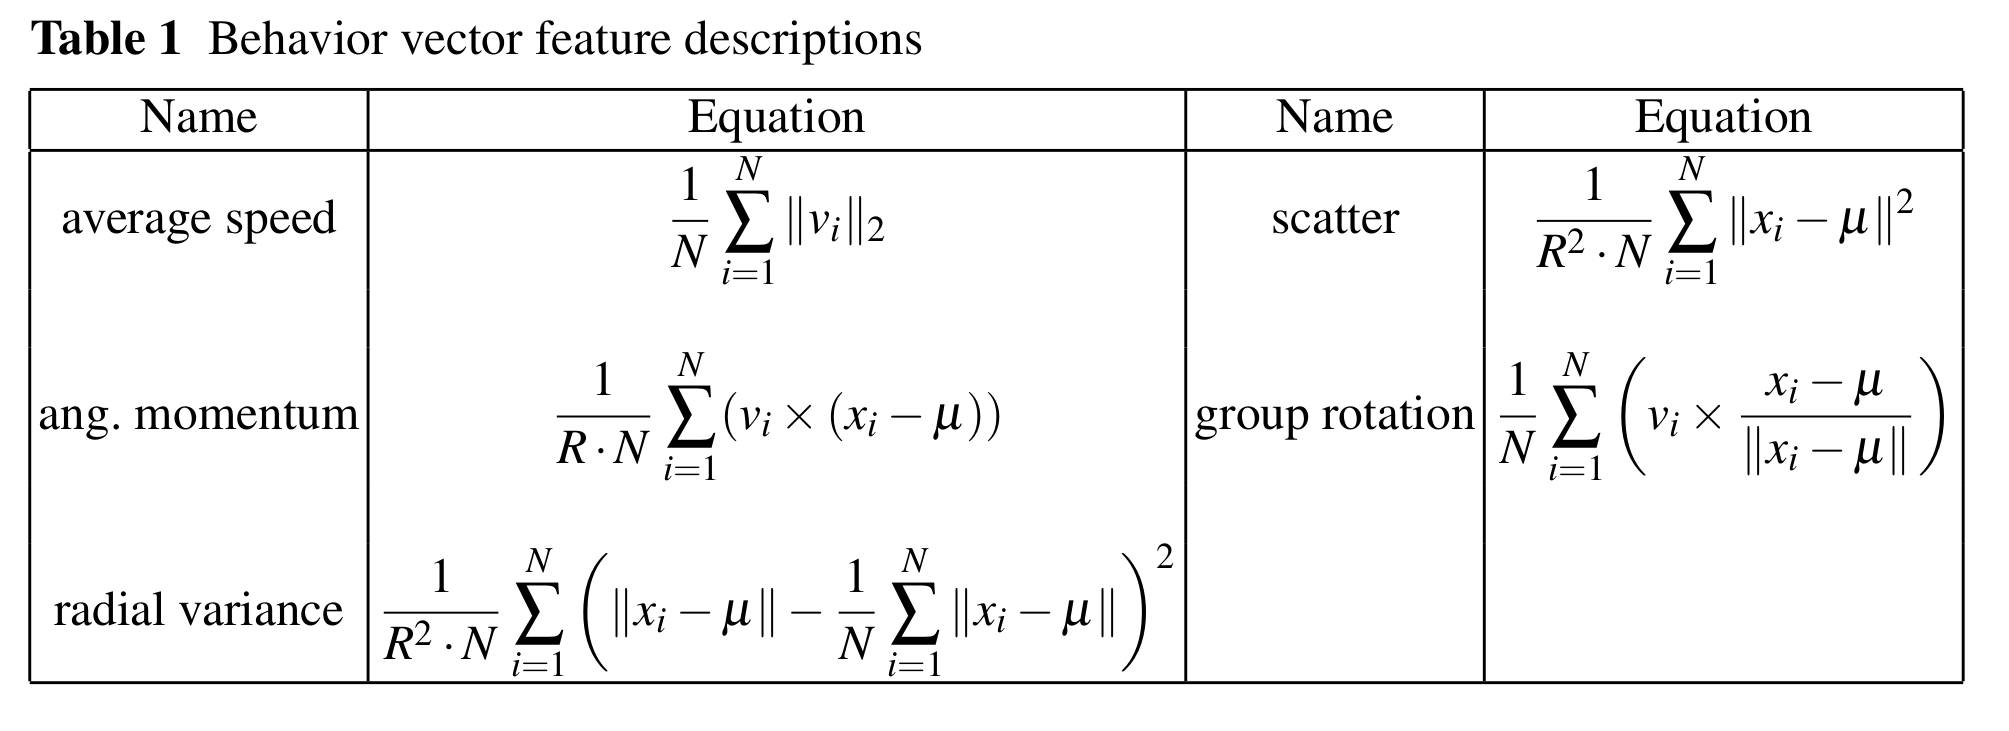
\includegraphics[width=\linewidth]{imgs/measures.png}
    \caption{Behavior Vector, Table 1 in Brown et. al.\cite{c1}}
    \label{fig:vec}
\end{figure}

\begin{lstlisting}[caption={Search algorithm (Python)}, label={lst:search}, language=Python, breaklines=true]

# Details at 
# github.com/SaahilClaypool/swarm_novelty_search/blob/master/search.py
def search():
    print("iteration, population, weights, segregation")
    seed = Observation([0.5, 0.5, 0.5, .5, .5, .5])
    population = [seed]
    archive = []
    stop = False
    it = 0
    max_it = 100
    while(max_it != 0):
        it += 1
        max_pop = -1
        for idx, p in enumerate(population):
            _features = p.getMeasures()
            global PRIOR_WEIGHTS
            PRIOR_WEIGHTS.append(p.weights)
            if (shouldAddToArchive(p, p, archive)):
                archive.append(p)

        population = updatePopulation(population, archive)

        max_it -= 1

    seg = most_segregated(archive)
    print("most segregated\n", seg)

\end{lstlisting}

\subsection{Time Complexity}
\label{sec:time}

The obstacle in our implementation is the time complexity involved in the evoluationary search.
By increasing the number of weights in our model from 4 to 6, we increased the search space from 4 dimmensions to 6. 
In our original implemntation, we were fully permutating each weight vector.
That is, for each population we would test \emph{all possible combinations} of increased or decreasing the weights in the vector. 
For example, if the weights of a two dimmensional vector were \texttt{[.1, .2]}, and the step size\footnote{We use a step size of .1, and bound each weight between 0 and 1.}, then a single permutation of this population would create the following new populations
\begin{itemize}
    \item \texttt{[.0, .1]}
    \item \texttt{[.0, .2]}
    \item \texttt{[.0, .3]}
    \item \texttt{[.1, .1]}
    \item \texttt{[.1, .3]}
    \item \texttt{[.2, .1]}
    \item \texttt{[.2, .2]}
    \item \texttt{[.2, .3]}
\end{itemize}

Which is $3^2 - 1 = 8$ new populations. 
This is because each value can either increase, decrease, or stay the same. 
So, for each new weight added, three new populations can be generated. 
This meant that when we created a 6-weight neural network, each population could generate a potential of $3^6 - 1$ populations, or 728 new populations.
Each population takes roughly 10 to 30 seconds to simulate in our implementation, causing each generation of the evolutionary search to take roughly 6 hours on a relatively powerful machine. 

Thus, we needed to adjust our implementation to reduce this time complexity. 
We did this with two different approaches. 
Our first approach was to return to a 4 weight model, but change the semantics of our simulation such that weights 1 and 2 were used only if a robot of the \emph{same} time was visible directly infront of the current robot.
Otherwise, the other two weights would be used whether there was no robot infront of the current robot, or a robot of the other type. 
This made the bots effectively blind to bots of the wrong type, but from our experimenting, it seems that well-segregated swarms would often just turn away from swarms of the oher type.
Thus, the swarms of the other type would not be in `line of sight' for more than a single time step, and thus the weights controlling the behavior when a bot of the other type is visible were rarely used. 
So, we combined these weights with the weights controlling the behavior when no bot is visible. 

Our second heuristic was to \emph{not} compute all combinations of the weights for the current population, but rather just increase each weight individually to create new populations. 
This reduces the number of new populations generated each generation from $3^W - 1$ to $3 \times W - 1$. 
In the case of our 6-weight example, this reduces the number of permutations from 728 to just 17. 
This makes each generation less effective, but made each iteration exponentially faster. 
This allowed us to run the same experiment with all 6 weights being evaluated. 
In the results, we will discuss the differences discovered by these two approaches.


\subsubsection{Fitness Search vs Novelty Search}

Unlike Brown et. al., we do not aim to categorize the complete set of possible behaviors given a limited capability model. 
Rather, we aim to answer just one question: given this capability model (4 to 6 neuron network, differential drive motor, binary line of sight, same-swarmm detection) is the behavior of segregation possible. 
Thus, a novelty is not necessarily the best fitness function - novelty is useful for ensuring our algorithm covers all parts of the search space, but that is not our aim. 
Thus we also implement a second search that replaces novelty with a traditional fitness function.
The semantics of the algorithm are unchanged. 
The only change is as follows: rather than selecting the most unique population to permutate in the next generation, we instead choose the population which exhibited the highest levels of segregation.


\subsection{Segregation Metrics}

To evaluate which population exhibited the highest levels of segregation, we created a quantifiable measure of segregation. 
To be a valid measure of segregation, this measure should have the following properties: 
\begin{itemize}
    \item Higher segregation should correspond to higher segregation measure scores

        For ease of interpretability, the measure should \emph{maximize} segregation when two groups are completely split.

    \item Groups with low segregation scores should correspond to groups that are indistinguishable from each other

        If two groups were to not segregate, that would likely mean they were interspersed evenly within each other. 
        Similarly, if two groups are interspersed evenly within each other, they are not segregated. 

\end{itemize}

Thus, the metric we use is as follows:

$$
({\frac{DistanceDeviation_1 + DistanceDeviation_2}{2 DistanceDeviation}})^{-1}
$$

Where the distance $DistanceDeviation$ is the standard deviation of all the bots to the mean position of all of the bots, $DistanceDeviation_1$ is the standard deviations of the distance of all the bots to the center of mass of that group, and $DistanceDeviation_2$ is the same for group 2. 

The reasoning for this measure is that, when the groups are overlapping, the standard deviation within a single group should be the same as the standard deviation of the entire set of robots. 
Thus the term $\frac{DistanceDeviation_1 + DistanceDeviation_2}{2 DistanceDeviation}$ should be roughly equal to 1. 
But, when the groups are highly segregated, $DistanceDeviation_1$ and $DistanceDeviation_2$ should be smaller than $DistanceDeviation$. 
Thus, the term should tend towards zero. 
Because we take the inverse, this measure should get larger when the bots are segregated. 
We provide validation and discussion on this measure of segregation in the next section.

\section{Results}
\label{sec:res}

This section is structured as follows: First, Section~\ref{sec:seg4} demonstrates the level of segregation that can occur given our limited capability model with 4 neurons; Section~\ref{sec:seg6} demonstrates the behavior of a 6 neuron model; finally, Section~\ref{sec:fitness} discusses the performance our fitness search model. 


\subsection{Segregation with 4-neuron capability model}
\label{sec:seg4}

Our key contribution is to determine whether we can observe segregation with our given capability model. 
To determine this, we the previously described novelty search algorithm for 100 generations.
During each generation, we tested \emph{all permutations} of the 4 neuron weights with a step size of 0.1, which ensures that each step discover the true `most novel' new population.

At the end of this process, the population which demonstrated the highest segregation score had the weights $[0.61, 0.59, 0.01, 0.3]$. 
This can be interpreted as follows: when bot \emph{A} sees bot \emph{B} of the same type, it uses the first weights 0.61 and 0.59 to control its wheels.
This results in bot \emph{A} quickly moving generally straight (with a slight turn) towards the bot \emph{B}. 
When bot \emph{A} sees either nothing \emph{or} a bot of any other type, then the bot will use the second set of weights, 0.1, 0.3, to control its left and right wheels respectively. 
This results in the bot mostly spinning in place until it sees a bot of the same type. 

This behavior can be seen in Figure~\ref{fig:init_pos_1} which depicts the positions of the bots over the course of the simulation. 
The colored depict the location of the bots at the start of the simulation and the light colored paths depict the locations of where the bots will travel. 
As seen here, the bots are evenly dispersed at the start of the simulation, and thus not segregated.
The circling behavior can be seen at locations $X= 0$, $Y= -1.5$. 
The paths of the bots are drawn with low opacity, so the dark circle here demonstrates that a bot spent a great deal of time circling this location. 


\begin{figure}
    \centering
    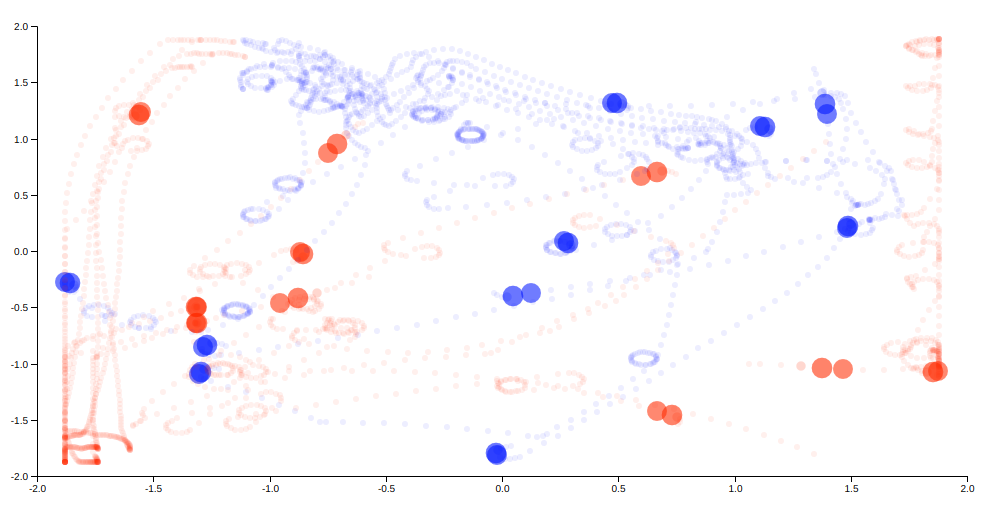
\includegraphics[width=\linewidth]{imgs/init_place_1.png}
    \caption{Positions of bots at the start of the simulation}
    \label{fig:init_pos_1}
\end{figure}

Figure~\ref{fig:final_seg_1} depicts our calculated segregation score for this population during each iteration. 
The highest segregation can be seen around step 2,400. 
The three values used to calculate this metric over the same time period are shown in Figure~\ref{fig:final_dev_1}. 
The line represent the standard deviation of the distances from the bots to the metroid of the cluster for each swarm with red line corresponding to the red group, the blue corresponding to the blue group, and the gray line corresponding to the total standard deviation of distances to the center of all bots. 
The dark colored dot depicts the current time in our animation~\footnote{We use an interactive animation to depict these results. Github:

\url{http://tiny.cc/e4hv5y}}.
Figure~\ref{fig:final_pos_1} demonstrates the location of the bots during this point of highest segregation. 
As expected, when the bots look visually segregated, the intra-group standard deviations of their positions are low and the inter-group deviations are high (Figure~\ref{fig:final_dev_1}), and this corresponds to a high numeric value of segregation (Figure~\ref{fig:final_seg_1}). 

\begin{figure}
    \centering
    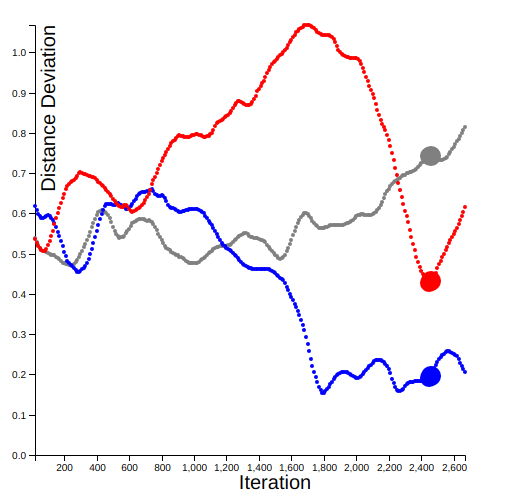
\includegraphics[width=5.5cm]{imgs/final_dev_1.png}
    \caption{Standard deviations of inter and intra-group distances for each population}
    \label{fig:final_dev_1}
\end{figure}

\begin{figure}
    \centering
    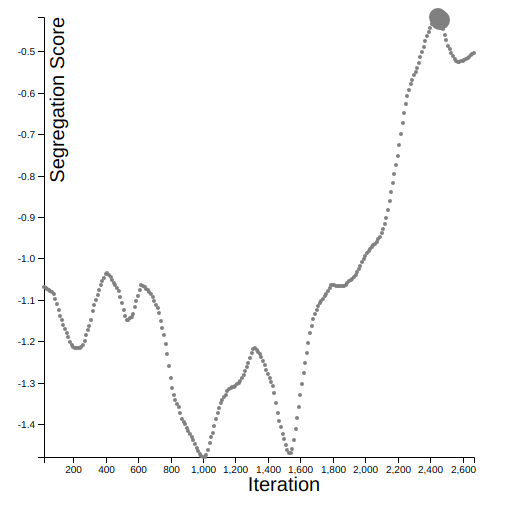
\includegraphics[width=5.5cm]{imgs/final_seg_1.png}
    \caption{Segregation score of the population at each time step}
    \label{fig:final_seg_1}
\end{figure}

\begin{figure}
    \centering
    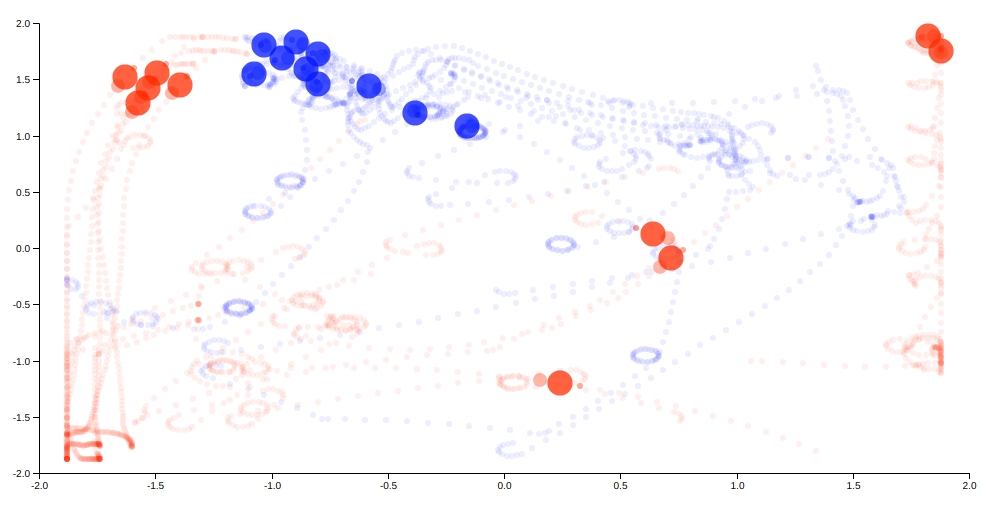
\includegraphics[width=\linewidth]{imgs/final_place_1.png}
    \caption{Positions of bots at the location of the highest clustering}
    \label{fig:final_pos_1}
\end{figure}

\subsection{Dispersion test}
\label{sec:dispersion}

To validate our segregation metrics, we hand-coded a population that would create high dispersal. 
We did this by setting the weights to $[0.3, 0.3, 0.3, 0.3, 0.3, 0.3]$.
Using these weights, the bots would \emph{always} move straight forward at a slow speed.
The results for this format can be seen in Figures~\ref{fig:final_dev_d}, \ref{fig:final_seg_d}, and \ref{fig:final_pos_d} depict the results in a similar format to the above images. 
As seen here, the bots move straight until they reach the edge of the map, at which point they continue to move straight but are largely stationary. 
Thus, the standard deviation in the positions (Figure\ref{fig:final_dev_d}) remains fairly uniform across all of the clusters - there is no extra clustering between groups of the same type. 
The segregation score depicted in \ref{fig:final_seg_d} also remains very low, reflecting the low preference for segregation exhibited by this population.
This serves as a sort of validation that our segregation metric is able to discriminate against poorly segregated populations, and that our capability can still exhibit some forms of segregations.

\begin{figure}
    \centering
    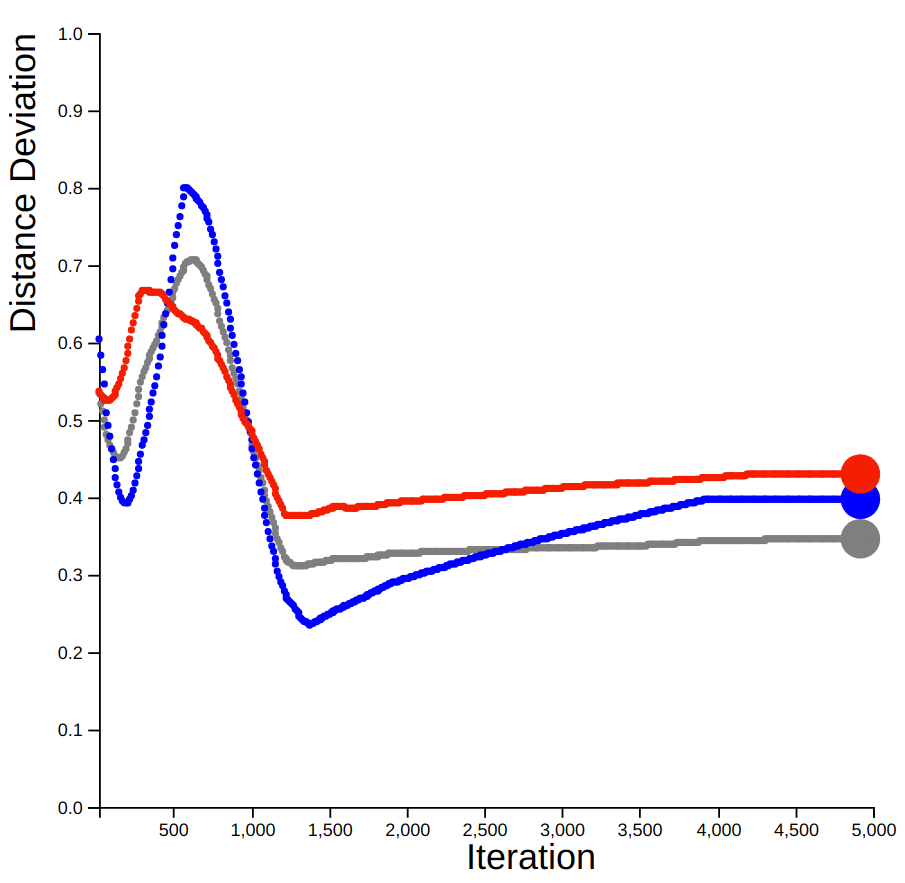
\includegraphics[width=5.5cm]{imgs/final_dev_d.png}
    \caption{Standard deviations of inter and intra-group distances for each cluster of high-dispersal population}
    \label{fig:final_dev_d}
\end{figure}

\begin{figure}
    \centering
    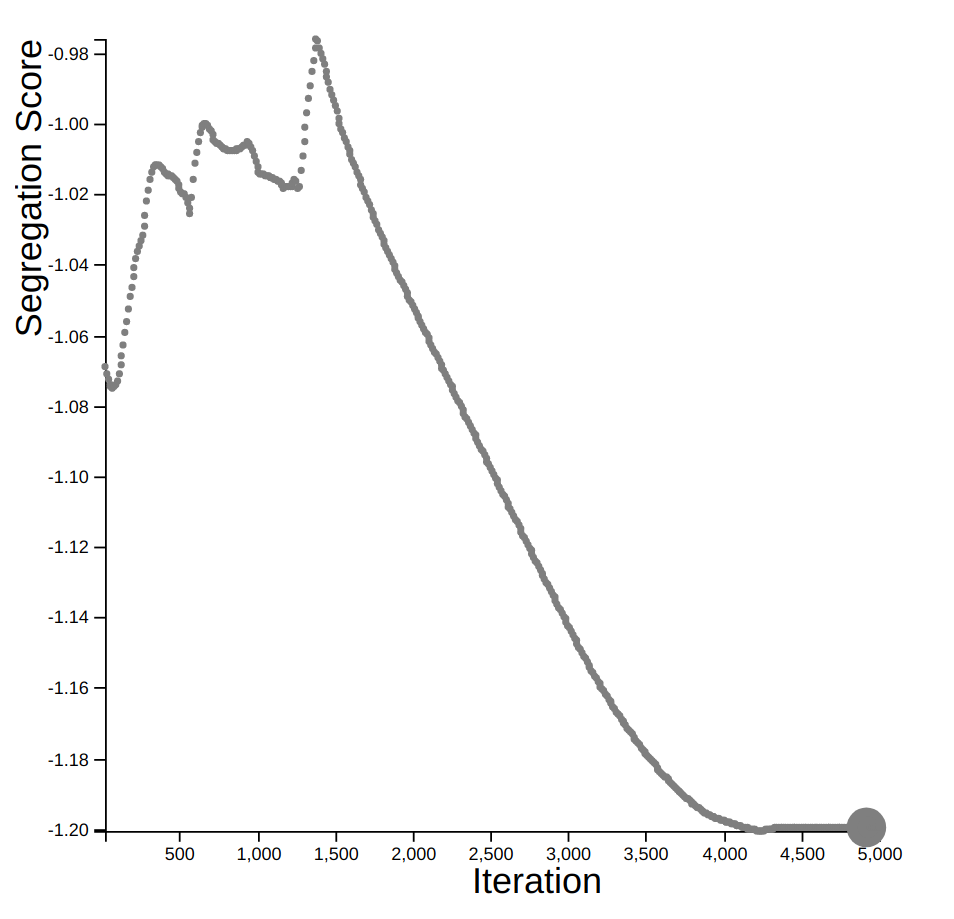
\includegraphics[width=5.5cm]{imgs/final_seg_d.png}
    \caption{Segregation score of the population at each time step for high-dispersal population}
    \label{fig:final_seg_d}
\end{figure}

\begin{figure}
    \centering
    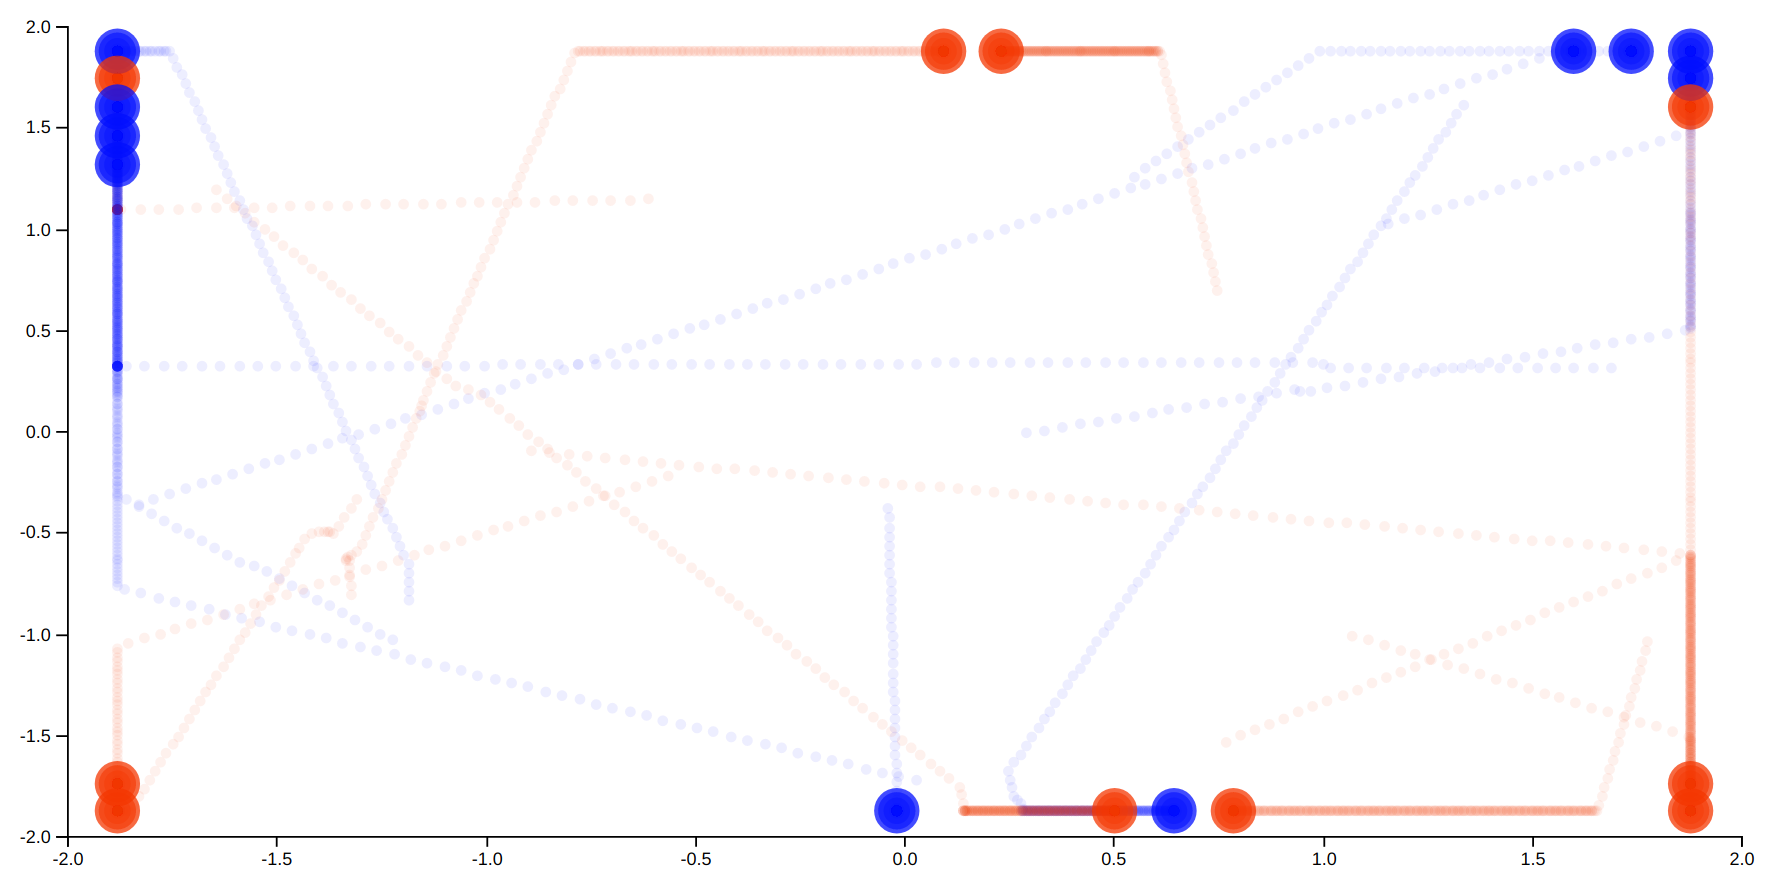
\includegraphics[width=\linewidth]{imgs/final_place_d.png}
    \caption{Positions at the end of the simulation for high dispersal population}
    \label{fig:final_pos_d}
\end{figure}



\subsection{Segregation with 6-neuron capability model}
\label{sec:seg6}



\subsection{Fitness search performance}
\label{sec:fitness}

After running the experiments above, we determined that a novelty search is not the most efficient technique for our problem. 
Where a novelty search worked well for Brown et. al. who were trying to categorize \emph{all} possible behaviors exhibited by the capability model, we were only interested in determining one behavior - segregation.
And, as we already determined a valid measure of segregation for our model, we were able to refit our evolutionary search using a fitness function that favors segregation instead of novelty. 
Thus, at each generation of the evolutionary search, we sort the new populations by their segregation scores. 
Then, rather than permuting the most novel population from these new populations, we instead permute the most segregated population.

After 100 generations, the most segregated population has the weights $[0.56, 0.46, 0.21, 0.31]$, which is slightly different from the most segregated population discovered by the original novelty search. 
The behavior of this population is summarized in the above format in Figures~\ref{fig:final_dev_2}, \ref{fig:final_seg_2}, and \ref{fig:final_pos_2}. 
As seen in Figure~\ref{fig:final_seg_2}, the segregation for this population is high, peaking at around $-0.6$, which is slightly higher than the highest segregation exhibited by the best novelty search result. 

We also plot the highest segregation of each generation in Figure~\ref{fig:fitness_search}. 
In general, each generation is able to find a better segregating population than the previous, and this seems to have diminishing returns as the simulation goes on\footnote{Note that this function is roughly bounded between zero and one, so it must have asymptotic functions over time}. 
Also, as seen in the previous sections, the segregation scores for the populations is not very stable, and it can fluctuate greatly between each time step for a single population. 
To generate this figure, we took the last time step's segregation score, which may not have been the highest segregation score exhibited over the course of that population's runtime. 

\begin{figure}
    \centering
    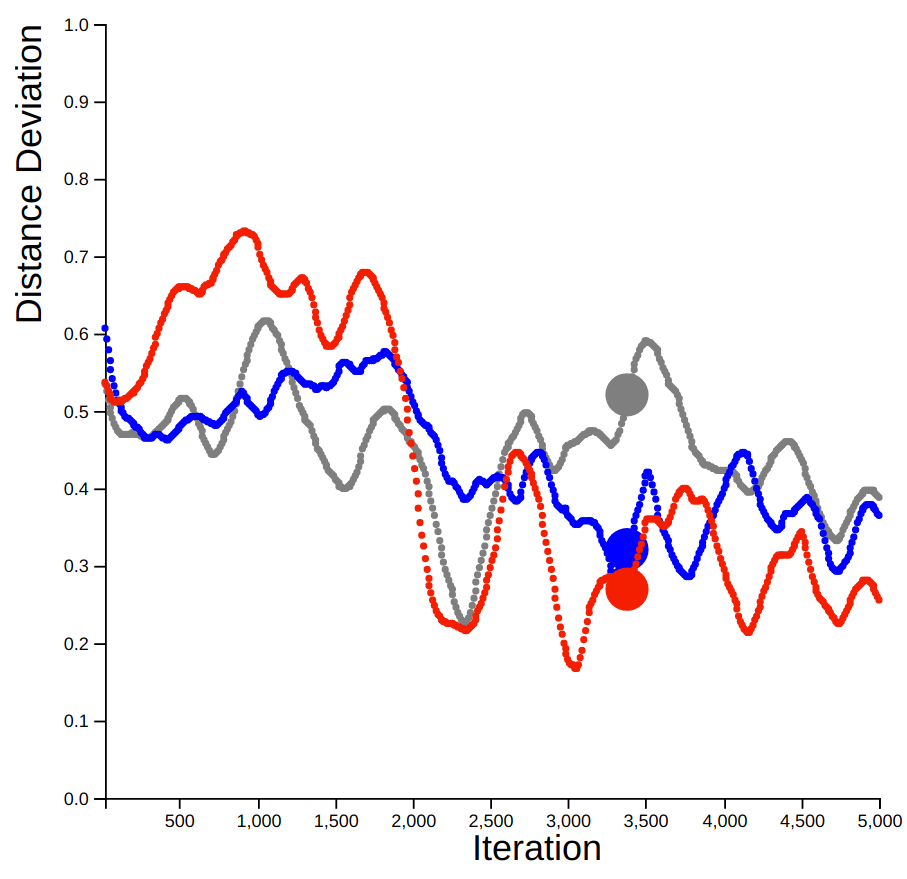
\includegraphics[width=5.5cm]{imgs/final_dev_2.png}
    \caption{Standard deviations of inter and intra-group distances for each robot in fitness search population}
    \label{fig:final_dev_2}
\end{figure}

\begin{figure}
    \centering
    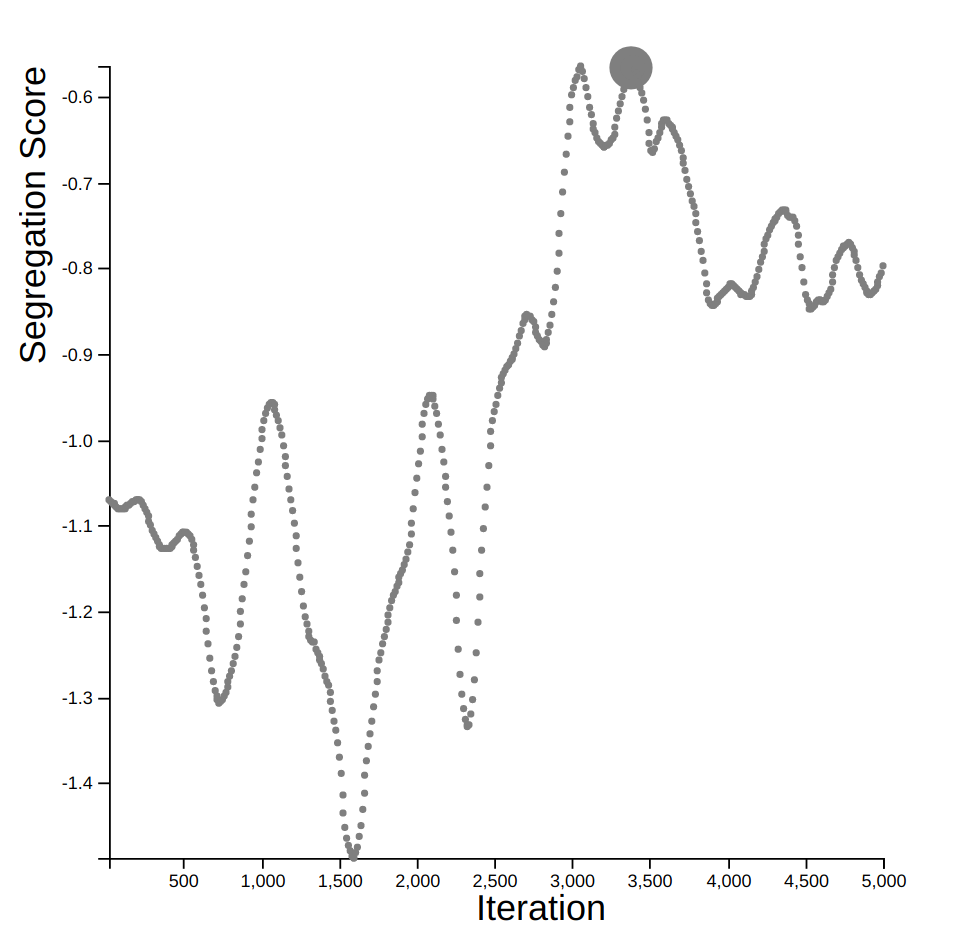
\includegraphics[width=5.5cm]{imgs/final_seg_2.png}
    \caption{Segregation score of the population at each time step in fitness search population}
    \label{fig:final_seg_2}
\end{figure}

\begin{figure}
    \centering
    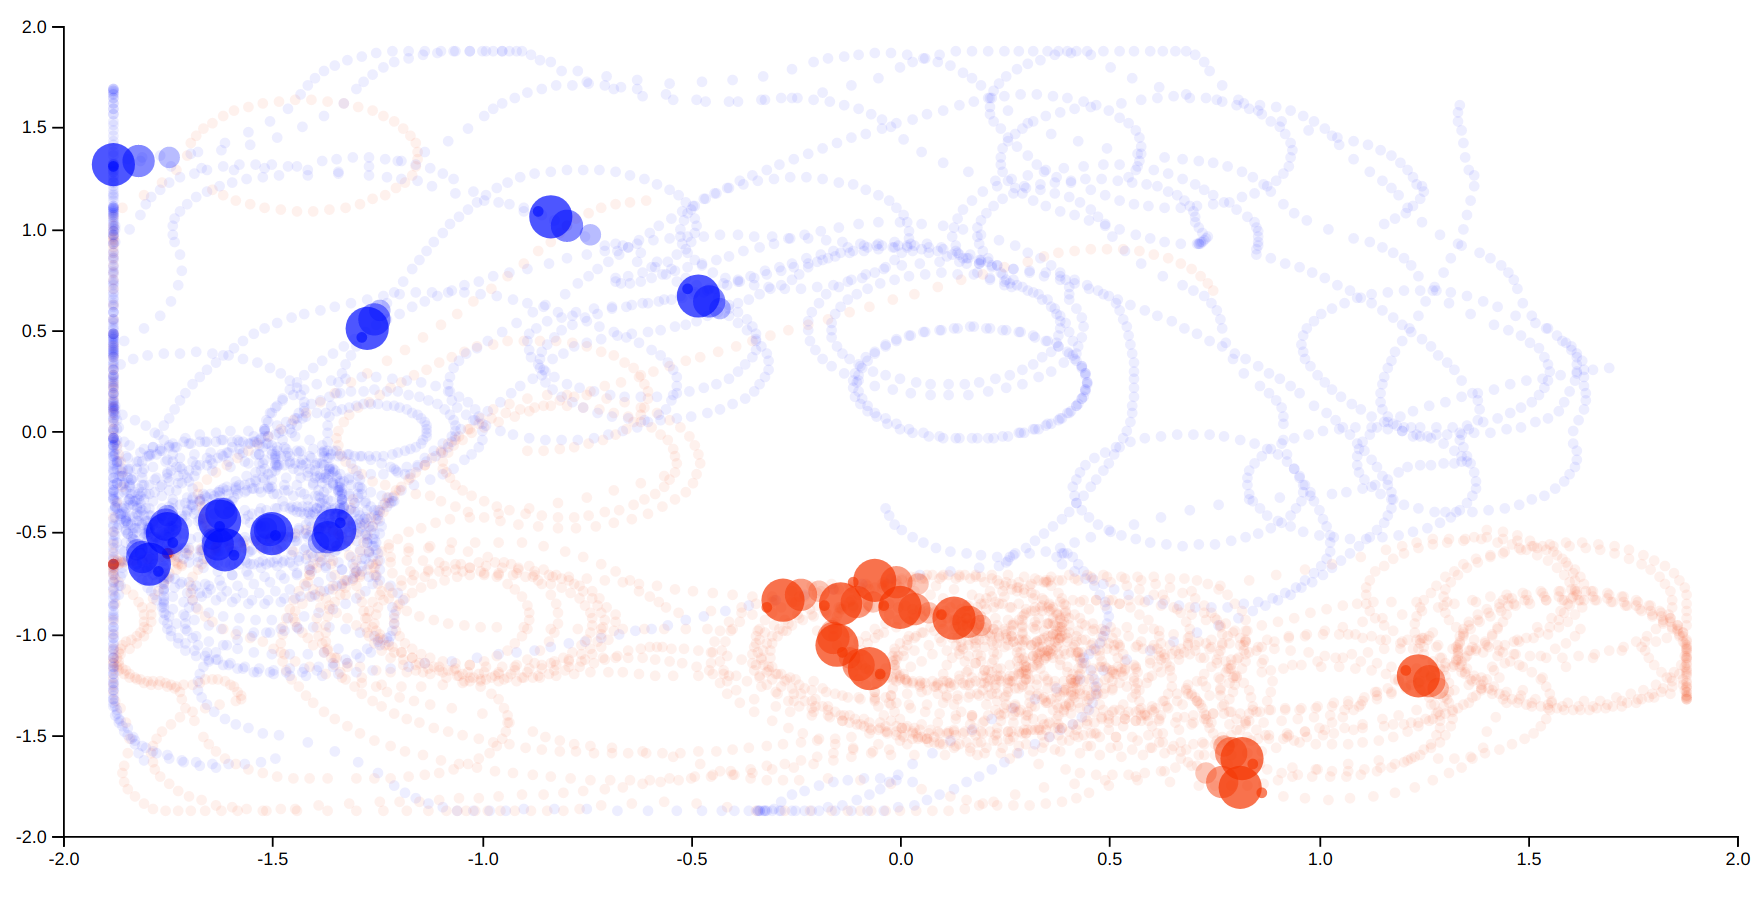
\includegraphics[width=\linewidth]{imgs/final_place_2.png}
    \caption{Positions of bots at the location of the highest clustering in fitness search population}
    \label{fig:final_pos_2}
\end{figure}

\begin{figure}
    \centering
    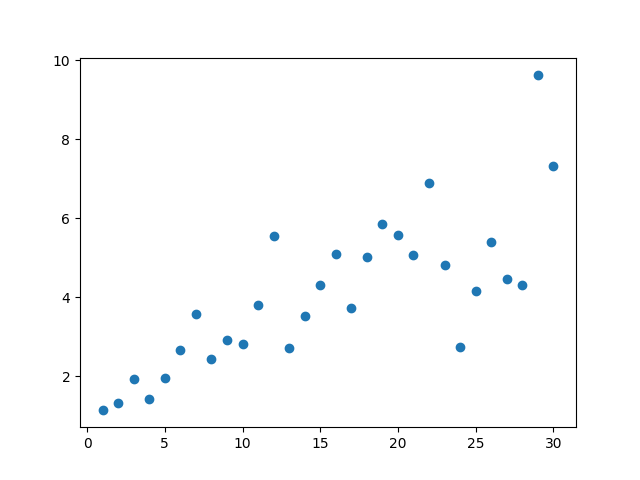
\includegraphics[width=\linewidth]{imgs/fitness_search.png}
    \caption{Maximum fitness observed in each generation}
    \label{fig:fitness_search}
\end{figure}

\input{discussion.tex}

% \subsection{Units}
% \begin{itemize}
% \item Use either SI (MKS) or CGS as primary units. (SI units are encouraged.) English units may be used as secondary units (in parentheses). An exception would be the use of English units as identifiers in trade, such as ``3.5-inch disk drive''.
% \item Avoid combining SI and CGS units, such as current in amperes and magnetic field in oersteds. This often leads to confusion because equations do not balance dimensionally. If you must use mixed units, clearly state the units for each quantity that you use in an equation.
% \item Do not mix complete spellings and abbreviations of units: ``Wb/m\textsuperscript{2}'' or ``webers per square meter'', not ``webers/m\textsuperscript{2}''. Spell out units when they appear in text: ``. . . a few henries'', not ``. . . a few H''.
% \item Use a zero before decimal points: ``0.25'', not ``.25''. Use ``cm\textsuperscript{3}'', not ``cc''.)
% \end{itemize}

% sentence, as in:
% \begin{equation}
% a+b=\gamma\label{eq}
% \end{equation}

% Be sure that the 
% symbols in your equation have been defined before or immediately following 
% the equation. Use ``\eqref{eq}'', not ``Eq.~\eqref{eq}'' or ``equation \eqref{eq}'', except at 
% the beginning of a sentence: ``Equation \eqref{eq} is . . .''

% \subsection{\LaTeX-Specific Advice}

% Please use ``soft'' (e.g., \verb|\eqref{Eq}|) cross references instead
% of ``hard'' references (e.g., \verb|(1)|). That will make it possible
% to combine sections, add equations, or change the order of figures or
% citations without having to go through the file line by line.

% Please don't use the \verb|{eqnarray}| equation environment. Use
% \verb|{align}| or \verb|{IEEEeqnarray}| instead. The \verb|{eqnarray}|
% environment leaves unsightly spaces around relation symbols.

% Please note that the \verb|{subequations}| environment in {\LaTeX}
% will increment the main equation counter even when there are no
% equation numbers displayed. If you forget that, you might write an
% article in which the equation numbers skip from (17) to (20), causing
% the copy editors to wonder if you've discovered a new method of
% counting.

% {\BibTeX} does not work by magic. It doesn't get the bibliographic
% data from thin air but from .bib files. If you use {\BibTeX} to produce a
% bibliography you must send the .bib files. 

% {\LaTeX} can't read your mind. If you assign the same label to a
% subsubsection and a table, you might find that Table I has been cross
% referenced as Table IV-B3. 

% {\LaTeX} does not have precognitive abilities. If you put a
% \verb|\label| command before the command that updates the counter it's
% supposed to be using, the label will pick up the last counter to be
% cross referenced instead. In particular, a \verb|\label| command
% should not go before the caption of a figure or a table.

% Do not use \verb|\nonumber| inside the \verb|{array}| environment. It
% will not stop equation numbers inside \verb|{array}| (there won't be
% any anyway) and it might stop a wanted equation number in the
% surrounding equation.

% \subsection{Some Common Mistakes}\label{SCM}
% \begin{itemize}
% \item The word ``data'' is plural, not singular.
% \item The subscript for the permeability of vacuum $\mu_{0}$, and other common scientific constants, is zero with subscript formatting, not a lowercase letter ``o''.
% \item In American English, commas, semicolons, periods, question and exclamation marks are located within quotation marks only when a complete thought or name is cited, such as a title or full quotation. When quotation marks are used, instead of a bold or italic typeface, to highlight a word or phrase, punctuation should appear outside of the quotation marks. A parenthetical phrase or statement at the end of a sentence is punctuated outside of the closing parenthesis (like this). (A parenthetical sentence is punctuated within the parentheses.)
% \item A graph within a graph is an ``inset'', not an ``insert''. The word alternatively is preferred to the word ``alternately'' (unless you really mean something that alternates).
% \item Do not use the word ``essentially'' to mean ``approximately'' or ``effectively''.
% \item In your paper title, if the words ``that uses'' can accurately replace the word ``using'', capitalize the ``u''; if not, keep using lower-cased.
% \item Be aware of the different meanings of the homophones ``affect'' and ``effect'', ``complement'' and ``compliment'', ``discreet'' and ``discrete'', ``principal'' and ``principle''.
% \item Do not confuse ``imply'' and ``infer''.
% \item The prefix ``non'' is not a word; it should be joined to the word it modifies, usually without a hyphen.
% \item There is no period after the ``et'' in the Latin abbreviation ``et al.''.
% \item The abbreviation ``i.e.'' means ``that is'', and the abbreviation ``e.g.'' means ``for example''.
% \end{itemize}
% An excellent style manual for science writers is \cite{b7}.

% \subsection{Authors and Affiliations}
% \textbf{The class file is designed for, but not limited to, six authors.} A 
% minimum of one author is required for all conference articles. Author names 
% should be listed starting from left to right and then moving down to the 
% next line. This is the author sequence that will be used in future citations 
% and by indexing services. Names should not be listed in columns nor group by 
% affiliation. Please keep your affiliations as succinct as possible (for 
% example, do not differentiate among departments of the same organization).

% \subsection{Identify the Headings}
% Headings, or heads, are organizational devices that guide the reader through 
% your paper. There are two types: component heads and text heads.

% Component heads identify the different components of your paper and are not 
% topically subordinate to each other. Examples include Acknowledgments and 
% References and, for these, the correct style to use is ``Heading 5''. Use 
% ``figure caption'' for your Figure captions, and ``table head'' for your 
% table title. Run-in heads, such as ``Abstract'', will require you to apply a 
% style (in this case, italic) in addition to the style provided by the drop 
% down menu to differentiate the head from the text.

% Text heads organize the topics on a relational, hierarchical basis. For 
% example, the paper title is the primary text head because all subsequent 
% material relates and elaborates on this one topic. If there are two or more 
% sub-topics, the next level head (uppercase Roman numerals) should be used 
% and, conversely, if there are not at least two sub-topics, then no subheads 
% should be introduced.

% \subsection{Figures and Tables}
% \paragraph{Positioning Figures and Tables} Place figures and tables at the top and 
% bottom of columns. Avoid placing them in the middle of columns. Large 
% figures and tables may span across both columns. Figure captions should be 
% below the figures; table heads should appear above the tables. Insert 
% figures and tables after they are cited in the text. Use the abbreviation 
% ``Fig.~\ref{fig}'', even at the beginning of a sentence.

% \begin{table}[htbp]
% \caption{Table Type Styles}
% \begin{center}
% \begin{tabular}{|c|c|c|c|}
% \hline
% \textbf{Table}&\multicolumn{3}{|c|}{\textbf{Table Column Head}} \\
% \cline{2-4} 
% \textbf{Head} & \textbf{\textit{Table column subhead}}& \textbf{\textit{Subhead}}& \textbf{\textit{Subhead}} \\
% \hline
% copy& More table copy$^{\mathrm{a}}$& &  \\
% \hline
% \multicolumn{4}{l}{$^{\mathrm{a}}$Sample of a Table footnote.}
% \end{tabular}
% \label{tab1}
% \end{center}
% \end{table}

% \begin{figure}[htbp]
% \centerline{\includegraphics{fig1.png}}
% \caption{Example of a figure caption.}
% \label{fig}
% \end{figure}

% Figure Labels: Use 8 point Times New Roman for Figure labels. Use words 
% rather than symbols or abbreviations when writing Figure axis labels to 
% avoid confusing the reader. As an example, write the quantity 
% ``Magnetization'', or ``Magnetization, M'', not just ``M''. If including 
% units in the label, present them within parentheses. Do not label axes only 
% with units. In the example, write ``Magnetization (A/m)'' or ``Magnetization 
% \{A[m(1)]\}'', not just ``A/m''. Do not label axes with a ratio of 
% quantities and units. For example, write ``Temperature (K)'', not 
% ``Temperature/K''.

% \section*{Acknowledgment}

% The preferred spelling of the word ``acknowledgment'' in America is without 
% an ``e'' after the ``g''. Avoid the stilted expression ``one of us (R. B. 
% G.) thanks $\ldots$''. Instead, try ``R. B. G. thanks$\ldots$''. Put sponsor 
% acknowledgments in the unnumbered footnote on the first page.

% \section*{References}

% Please number citations consecutively within brackets \cite{b1}. The 
% sentence punctuation follows the bracket \cite{b2}. Refer simply to the reference 
% number, as in \cite{b3}---do not use ``Ref. \cite{b3}'' or ``reference \cite{b3}'' except at 
% the beginning of a sentence: ``Reference \cite{b3} was the first $\ldots$''

% Number footnotes separately in superscripts. Place the actual footnote at 
% the bottom of the column in which it was cited. Do not put footnotes in the 
% abstract or reference list. Use letters for table footnotes.

% Unless there are six authors or more give all authors' names; do not use 
% ``et al.''. Papers that have not been published, even if they have been 
% submitted for publication, should be cited as ``unpublished'' \cite{b4}. Papers 
% that have been accepted for publication should be cited as ``in press'' \cite{b5}. 
% Capitalize only the first word in a paper title, except for proper nouns and 
% element symbols.

% For papers published in translation journals, please give the English 
% citation first, followed by the original foreign-language citation \cite{b6}.

% \begin{thebibliography}{00}
\bibliography{references}
\bibliographystyle{ieeetr}
% \bibitem{c1} Brown et al
% \bibitem{c2} Ame, C. Rivault, and J. Deneubourg, ``Cockroach aggregation based on strain odour recognition,''Animal Behav., vol. 68, pp. 793–801,2004.
% \bibitem{c3} A. B. Sendova-Franks, S. R. Scholes, N. R. Franks, and C. Melhuis,``Brood sorting by ants: Two phases and differential diffusion,'' AnimalBeh., vol. 68, pp. 1095–1106, 2004.
% \bibitem{c4} Segregation  of  Heterogeneous  Unitsin a Swarm of Robotic AgentsManish Kumar, Devendra P. Garg, and Vijay Kumar. TODO: these should all be moved to a bibtex
% \bibitem{c5} A  Minimalistic  Approach  to  Segregationin  Robot  SwarmsPeter Mitrano1, Jordan Burklund1, Michael Giancola1, Carlo Pinciroli1
% \bibitem{c6} Segregation of Multiple Heterogeneous Units in a Robotic SwarmVinicius Graciano SantosLuciano C. A. PimentaLuiz Chaimowicz

% \bibitem{b1} G. Eason, B. Noble, and I. N. Sneddon, ``On certain integrals of Lipschitz-Hankel type involving products of Bessel functions,'' Phil. Trans. Roy. Soc. London, vol. A247, pp. 529--551, April 1955.
% \bibitem{b2} J. Clerk Maxwell, A Treatise on Electricity and Magnetism, 3rd ed., vol. 2. Oxford: Clarendon, 1892, pp.68--73.
% \bibitem{b3} I. S. Jacobs and C. P. Bean, ``Fine particles, thin films and exchange anisotropy,'' in Magnetism, vol. III, G. T. Rado and H. Suhl, Eds. New York: Academic, 1963, pp. 271--350.
% \bibitem{b4} K. Elissa, ``Title of paper if known,'' unpublished.
% \bibitem{b5} R. Nicole, ``Title of paper with only first word capitalized,'' J. Name Stand. Abbrev., in press.
% \bibitem{b6} Y. Yorozu, M. Hirano, K. Oka, and Y. Tagawa, ``Electron spectroscopy studies on magneto-optical media and plastic substrate interface,'' IEEE Transl. J. Magn. Japan, vol. 2, pp. 740--741, August 1987 [Digests 9th Annual Conf. Magnetics Japan, p. 301, 1982].
% \bibitem{b7} M. Young, The Technical Writer's Handbook. Mill Valley, CA: University Science, 1989.
% \end{thebibliography}
% \vspace{12pt}
% \color{red}
% IEEE conference templates contain guidance text for composing and formatting conference papers. Please ensure that all template text is removed from your conference paper prior to submission to the conference. Failure to remove the template text from your paper may result in your paper not being published.
\end{document}
